% PLANTILLA APA7
% Creado por: Isaac Palma Medina
% Última actualización: 25/07/2021
% @COPYLEFT

% Fuentes consultadas (todos los derechos reservados):  
% Normas APA. (2019). Guía Normas APA. https://normas-apa.org/wp-content/uploads/Guia-Normas-APA-7ma-edicion.pdf
% Tecnológico de Costa Rica [Richmond]. (2020, 16 abril). LaTeX desde cero con Overleaf (1 de 3) [Vídeo]. YouTube. https://www.youtube.com/watch?v=kM1KvHVuaTY Weiss, D. (2021). 
% Formatting documents in APA style (7th Edition) with the apa7 LATEX class. https://ctan.math.washington.edu/tex-archive/macros/latex/contrib/apa7/apa7.pdf @COPYLEFT

%+-+-+-+-++-+-+-+-+-+-+-+-+-++-+-+-+-+-+-+-+-+-+-+-+-+-+-+-+-+-++-+-+-+-+-+-+-+-+-+

% Preámbulo
\documentclass[stu, 12pt, letterpaper, donotrepeattitle, floatsintext, natbib, helv]{apa7}
\usepackage[utf8]{inputenc}
\usepackage{comment}
\usepackage{marvosym}
\usepackage{graphicx}
\usepackage{float}
\usepackage[normalem]{ulem}
\usepackage[spanish]{babel} 
%\usepackage{titling}
\let\apasubparagraph\subparagraph
\let\subparagraph\paragraph
\usepackage[compact]{titlesec}
\let\subparagraph\apasubparagraph
\usepackage{hyperref}
\selectlanguage{spanish}
\useunder{\uline}{\ul}{}
\newcommand{\myparagraph}[1]{\paragraph{#1}\mbox{}\\}
\graphicspath{{./Images/}}
\titleformat{\section}{\normalfont\large\bfseries}{\thetitle. \quad }{0pt}{}[{ \titlerule[0.8pt]}]
\titleformat{\subsection}{\normalfont\bfseries}{}{}{}[]

% Portada

\begin{document}
\begin{titlepage}
    \centering
    \vfill
    \LARGE Laboratorio \#1\\
    \vskip2cm
    \large Diego Quirós Artiñano \\
    Universidad Nacional de Costa Rica \\
    EIF-202: Soporte Técnico \\ 
    Carolina Gómez Fernández \\
    20 de marzo, 2022 \\
    \vfill
    
\includegraphics[width = 0.4\textwidth]{UNA.png} \\
    \vfill
    \vfill
    % (autores separados, consultar al docente)
    % Manera oficial de colocar los autores:
    %\author{Autor(a) I, Autor(a) II, Autor(a) III, Autor(a) X}
\end{titlepage}

% Índices
\pagenumbering{roman}
    % Contenido
\renewcommand\contentsname{\largeÍndice}
\tableofcontents
\setcounter{tocdepth}{2}
\newpage
    % Figuras
%\renewcommand{\listfigurename}{\largeÍndice de fíguras}
%\listoffigures
%\newpage
    % Tablas
%\renewcommand{\listtablename}{\largeÍndice de tablas}
%\listoftables
%\newpage

% Cuerpo
\pagenumbering{arabic}

%------------------------------------------------------------------------------------
\section{Introducción}

En este laboratorio se van a resolver varios ejercicios de la ley de ohm. Después se va a revisar un video de YouTube sobre el tema de Electrónica Analógica y Digital.

%------------------------------------------------------------------------------------
\section{Parte 1 (Ejercicios de resistencia, voltaje e intensidad)}
En esta sección se resolverán ejercicios relacionados a circuitos. \\
\subsection{Ejercicio 1}
\noindent Encuentre la resistencia de una cocina que consume 3 amperios a una tensión de 120 voltios. \\
\[R = \frac{V}{I}\]
\[R = \frac{120}{3}\]
\[R = 40\Omega\]
\subsection{Ejercicio 2}
\noindent ¿Qué diferencia de potencial (voltaje) hay que aplicar a un reóstato de 30 ohmios para que circulen a través de él 5 amperios?
\[V = R \times I\]
\[V = 30 \times 5\]
\[V = 150V\]
\subsection{Ejercicio 3}
\noindent En el circuito de la figura, calcular la resistencia total y la intensidad 
\begin{itemize}
    \item La resistencia total se obtiene sumando cada resistencia
\end{itemize}
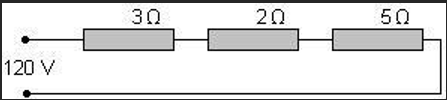
\includegraphics{Problem3.png}
\[R_T = 3\Omega + 2\Omega + 5\Omega\]
\[R_T = 10\Omega\]

\[I = \frac{V}{R}\]
\[I = \frac{120}{10}\]
\[I = 12A\]
\subsection{Ejercicio 4}
Un motor está construido para trabajar con una corriente de 3.5A a una diferencia de potencial de 115V. Este motor se instala en una red en la que la tensión es de 125V. Calcular el valor de la resistencia que hay que montar con el motor para conservar el valor previsto de la corriente. \\
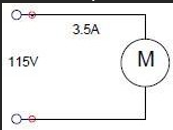
\includegraphics{Problem4.png}

\subsection{Ejercicio 5}
Una bombilla tiene la siguiente indicación: 220V - 100A. Calcula su resistencia.
\[R = \frac{V}{I}\]
\[R = \frac{220}{100}\]
\[R = 2.2\Omega\]

%----------------------------------------------------------------------------------------------------------------------------------
\section{Parte 2 (Resumen de video de Electrónica Analógica y Digital)}
\noindent \cite{video}\\
\begin{enumerate}
    \item Ver el video "Introducción a la Electrónica Analógica y Electrónica Digital" https://www.youtube.com/watch?v=TGozIvmanI8
    \item Realizar un resumen de los aspectos más importantes sobre la Electrónica Analógica y Digital.
\end{enumerate}

\noindent \textbf{Resumen:}
\begin{itemize}
    \item Electrónica: derivado de la electricidad que opera con elementos semi-conductores como microprocesadores, circuitos integrados y transistores.
    \item Analógica: voltajes continuos en el tiempo que tiene valores intermedio.
    \begin{itemize}
        \item Una radio vieja es análoga porque al mover el \textit{"dial"}, continuamente se cambia el número y se puede obtener cosas como 33.2.
        \item Componentes (Son importantes para entender como sirve y errores de un circuito):
        \begin {itemize}
            \item Resistor: se opone al flujo de corriente, lo regula y distribuye en un circuito, se mide en Ohmios ($\Omega$).
            \item Capacitor: acumula voltaje y lo libera al cargarse, puede servir como filtro reduciendo ruido de señales eléctricas, hay electrolíticos (definidos los positivos y negativos) o cerámicos (se puede conectar cualquiera de los dos lados en positivo y negativo), se mide en Faradios (F).
            \item Inductor (Bobina): acumula corriente y la libera cuando se requiere, minimiza ruido de señales eléctricas, su unidad de medida son los Henrys (H).
            \item Diodo: llega pasar la corriente por un lado y por el otro bloquea, es un semi-conductor hecho de cilicio o germanio, rectifica corrientes, algunos son reguladores de voltaje y otros de luces.
            \item Transistor: interruptor o amplificador de corriente, sus tres pines son: emisor, base y colector. 
        \end{itemize}
    \end{itemize}
    \item Digital: voltajes discretos, osea no continuos que tienen un valor definido.
    \begin{itemize}
        \item Una tableta es digital porque al tocar los botones de volumen se mueve tantas posiciones determinadas como de 30 a 40, pero no se puede tener 33.
        \item Parte del sistema de control de los aparatos electrónicos, dado a que operan con voltajes discretos o digitales.
        \item Estados lógicos: si un LED está prendido tiene 5 voltios y si apagado tiene 0 voltios (1 lógico y 0 lógico respectivamente)
        \item Familias circuitos digitales:
        \begin{itemize}
            \item TTL>: trabaja con 0 y 5 volts, circuitos basados en transistores BJT.
            \item CMOS: trabaja con 0 y 12 volts, circuits basados en transistores MOSFET (cambian de un estado lógico al otro con rapidez), sensibles a la electricidad estática (los puede quemar internamente, usar pulsera antiestática).
        \end{itemize}
        Las dos familias pueden trabajar con 1.5 o 3 volts como el 1 lógico.
        \item Los estados lógicos se combinan para hacer hardware digital como computadoras.
        \item Los estados lógicos se pueden usar a través de compuertas lógicas que el valor cambia dependiendo a los estados lógicos de entrada (Los más comunes son NOT, AND y OR), son la base de la electrónica digital.
        \item Flip-Flops: combinaciones de compuertas lógicas que forman circuitos que mantienen un estado lógico, son las memorias más simples, hay varios tipos y estos tienen diferentes resultados conforme los estados de entrada.
        \item Generador de pulsos: Los flip-flops son discretos y necesitan un cambio de estado en un tiempo determinado, generalmente un cristal de cuarzo, cuando se somete a presión emiten señales periódica millones de veces por segundo, haciendo que los procesadores sirvan adecuadamente.
        \item Señales periódicas: tienen dos características principales: la amplitud que es determinada por el voltaje de las ondas y la frecuencia es la ondas que pasan en un tiempo determinado (frecuencia de 20Mhz = 20 millones de ondas por segundo)
        \item circuitos integrados (chip): conjunto de miles de transistores compactados en microcircuitos, se fabrican en placas de material semi-conductoras (una o varias capas), compuertas simples o microprocesadores complejos. Funciones: almacenamiento de datos, transmisión de señales, procesamiento de instrucciones, entre otras. Todos traen hojas técnicas de especificaciones (detallando el trabajo de sus pines y detalles de operación)
    \end{itemize}
\end{itemize}

%----------------------------------------------------------------------------------------------------------------------------------------------------------------------
\section{Conclusión}
En este laboratorio se reforzaron los conocimientos sobre circuits y electrónica. Para hacer esto se resolvieron ejercicios y se resumió un video. Esto para fin de entender la relación que hay entre corriente, voltaje y resistencia, además de todos los diferentes componentes y aspectos que son requeridos al construir/arreglar algún dispositivo digital o analógico.
\newpage
% Referencias
\renewcommand\refname{\large\textbf{Referencias}}
\bibliography{mibibliografia}

\end{document}